\documentclass[11pt]{article} 
\usepackage[english]{babel}
\usepackage[utf8]{inputenc}
\usepackage[margin=0.5in]{geometry}
\usepackage{amsmath}
\usepackage{amsthm}
\usepackage{amsfonts}
\usepackage{amssymb}
\usepackage[usenames,dvipsnames]{xcolor}
\usepackage{graphicx}
\usepackage[colorinlistoftodos, color=orange!50]{todonotes}
\usepackage{hyperref}
\usepackage[numbers, square]{natbib}
\usepackage{fancybox}
\usepackage{epsfig}
\usepackage{soul}
\usepackage[framemethod=tikz]{mdframed}
\usepackage[shortlabels]{enumitem}
\usepackage[version=4]{mhchem}
\usepackage{multicol}
\usepackage{forest}
\usepackage{mathtools}
\usepackage{comment}
\usepackage{enumitem}
\usepackage[utf8]{inputenc}
\usepackage{listings}

\usepackage[numbers]{natbib}
\usepackage{subfiles}
\usepackage{algorithm}
\usepackage[noend]{algpseudocode}

\usepackage{tikz}
\usetikzlibrary{arrows.meta,positioning}

\tikzset{
	>=Stealth,            % arrow tip
	shorten >=2pt,        % trim arrow at head
	line width=0.5pt,
	node distance=2cm
}

\begin{document}
\title{CSCI 4302 Homework 3}
\author{Marcus Winton}
\maketitle
\section*{Policy Iteration}
Using policy iteration to solve the MDP problem given yields the following results, note the value of $\gamma$ used for these graphs is $\gamma = 0.99$. 
\begin{table}[H]
\centering
\begin{tabular}{ccc}
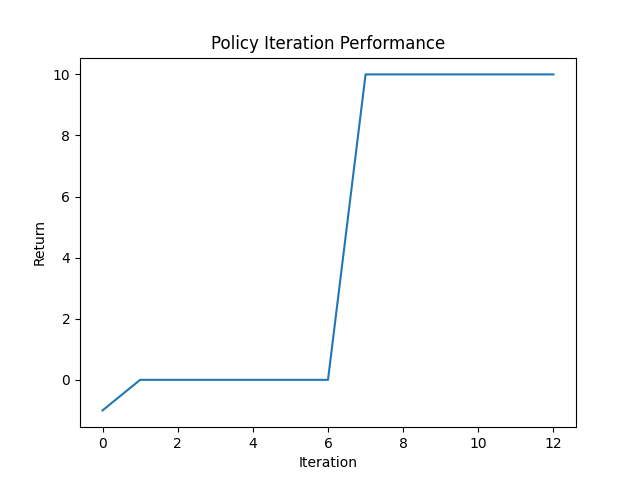
\includegraphics[scale=0.4]{hw4_rl/figures/gridworld-v0_deterministic_pi_gamma=0.99_curve} &
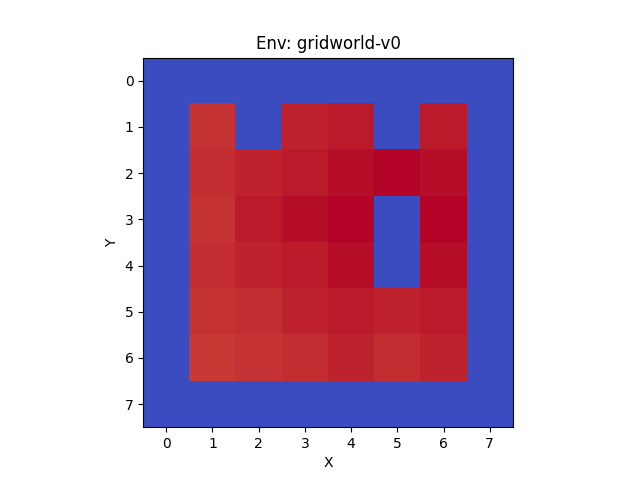
\includegraphics[scale=0.4]{hw4_rl/figures/gridworld-v0_deterministic_pi_gamma=0.99_value} &
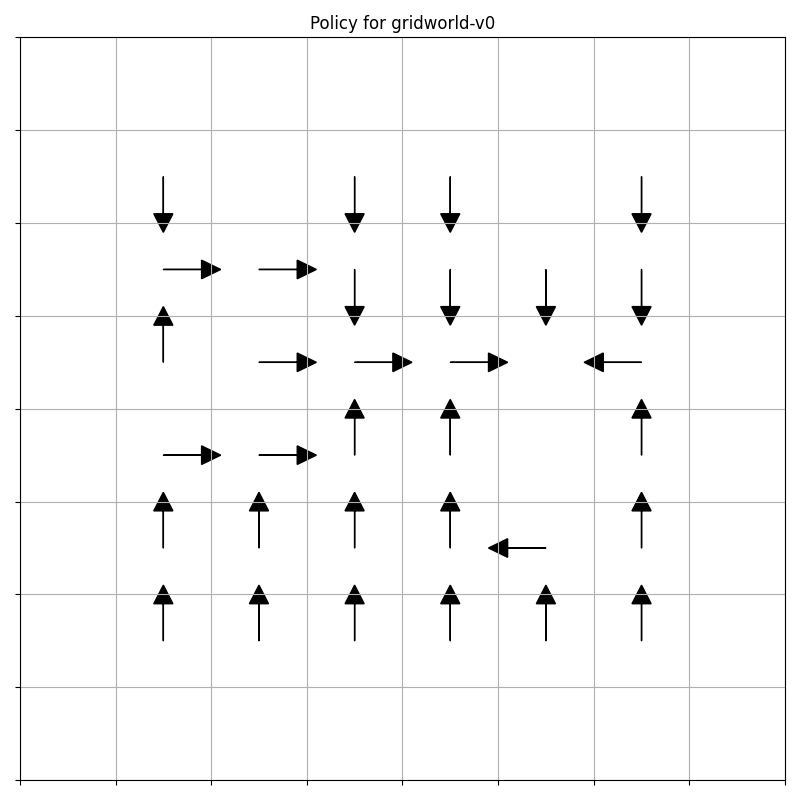
\includegraphics[scale=0.22]{hw4_rl/figures/gridworld-v0_deterministic_pi_gamma=0.99_policy}\\
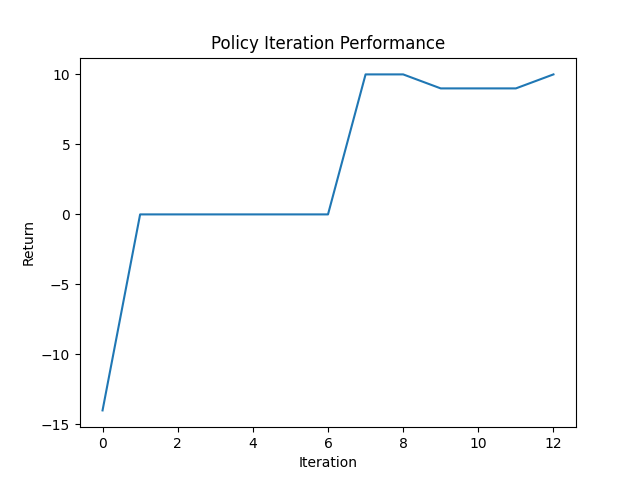
\includegraphics[scale=0.4]{hw4_rl/figures/gridworld-v1_deterministic_pi_gamma=0.99_curve} &
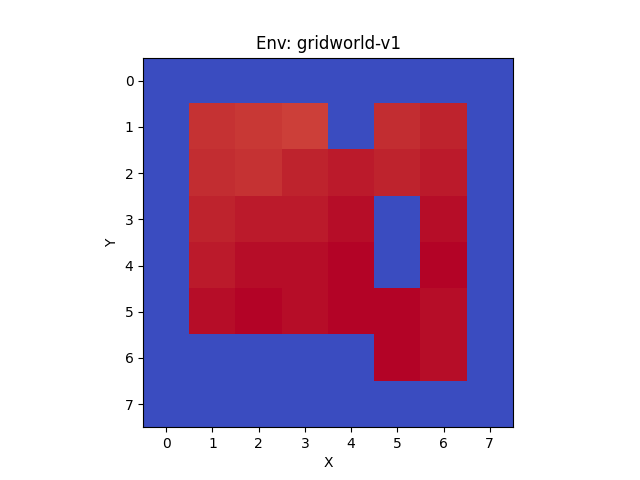
\includegraphics[scale=0.4]{hw4_rl/figures/gridworld-v1_deterministic_pi_gamma=0.99_value} &
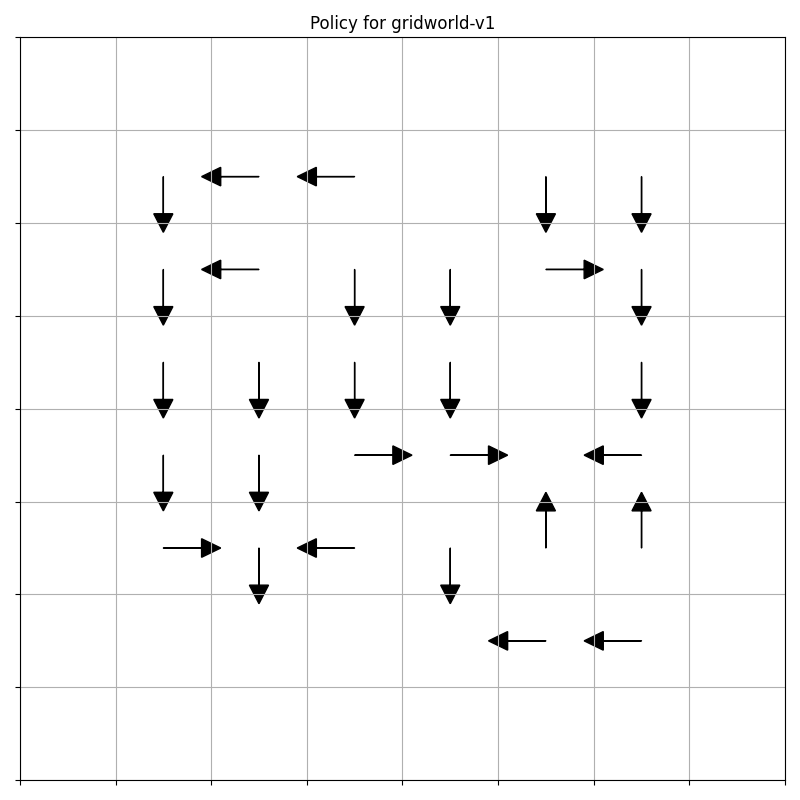
\includegraphics[scale=0.22]{hw4_rl/figures/gridworld-v1_deterministic_pi_gamma=0.99_policy}\\
Policy curve for each grid-world & Value heat-map for each grid-world &Policy graph for each grid-world
\end{tabular}
\caption{Graphs for the policy and value for each grid-world}
\label{tab:policy_itteration_curve_value_policy}
\end{table}
\newpage
Moving on to see how different values of $\gamma$ effect the policy, the table below shows the polices chosen for a given value of $\gamma$
\begin{table}[H]
\centering
\begin{tabular}{cccc}
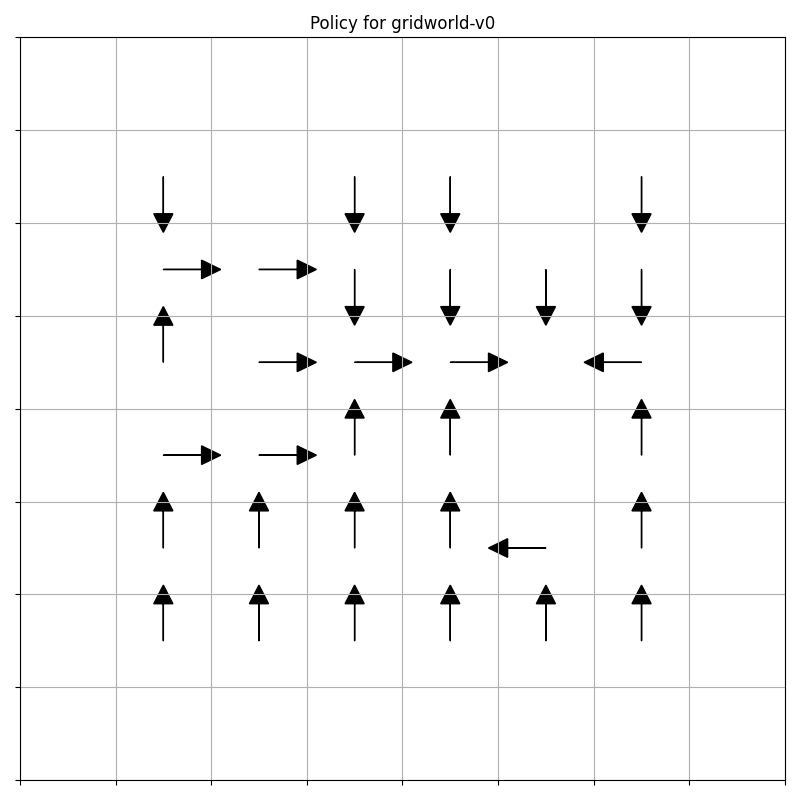
\includegraphics[scale=0.2]{hw4_rl/figures/gridworld-v0_deterministic_pi_gamma=0.5_policy} &
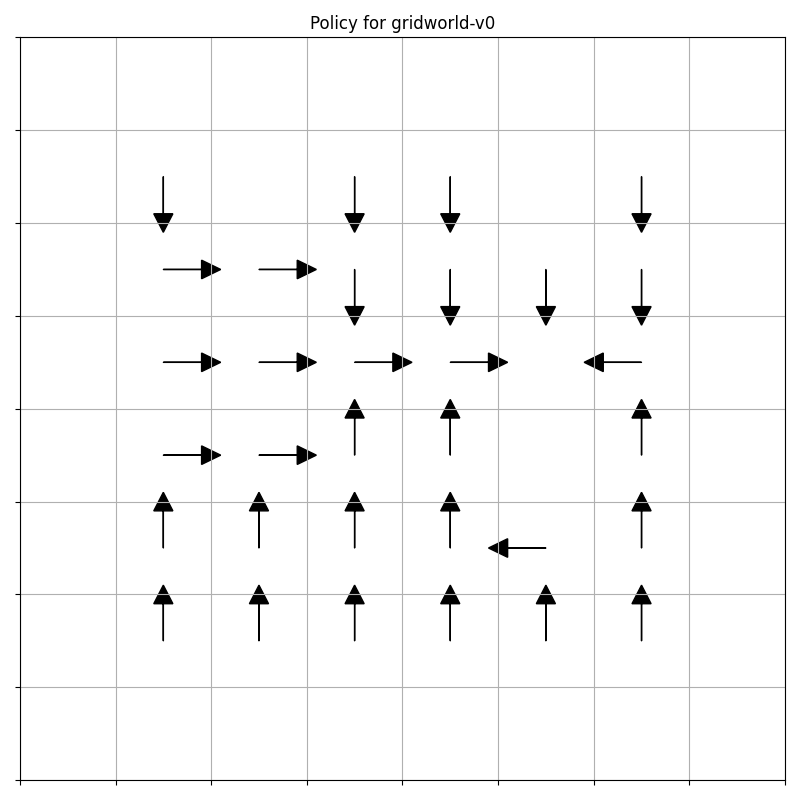
\includegraphics[scale=0.2]{hw4_rl/figures/gridworld-v0_deterministic_pi_gamma=0.75_policy} &
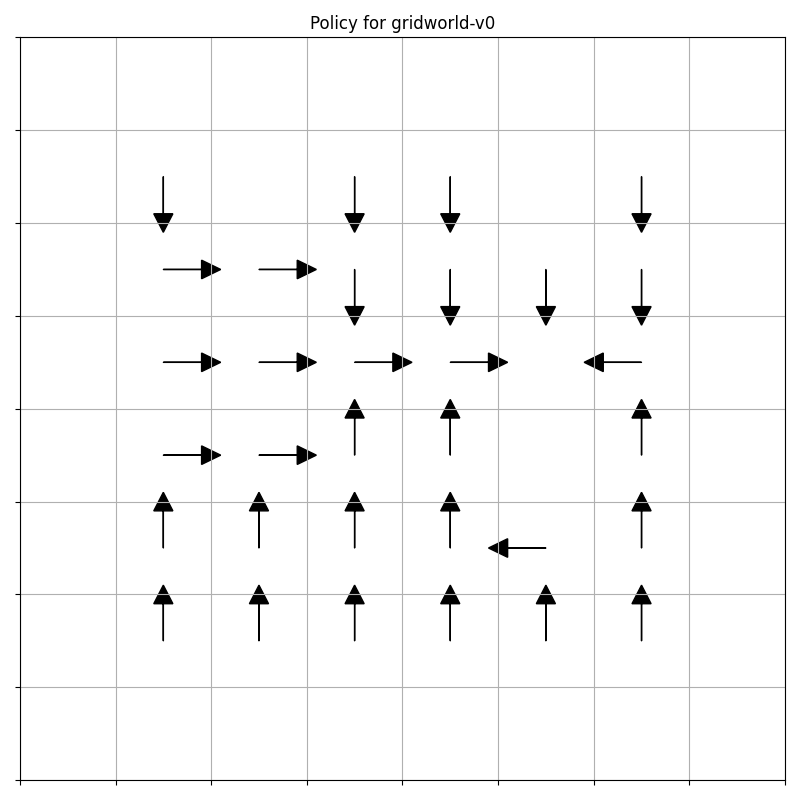
\includegraphics[scale=0.2]{hw4_rl/figures/gridworld-v0_deterministic_pi_gamma=0.9_policy} &
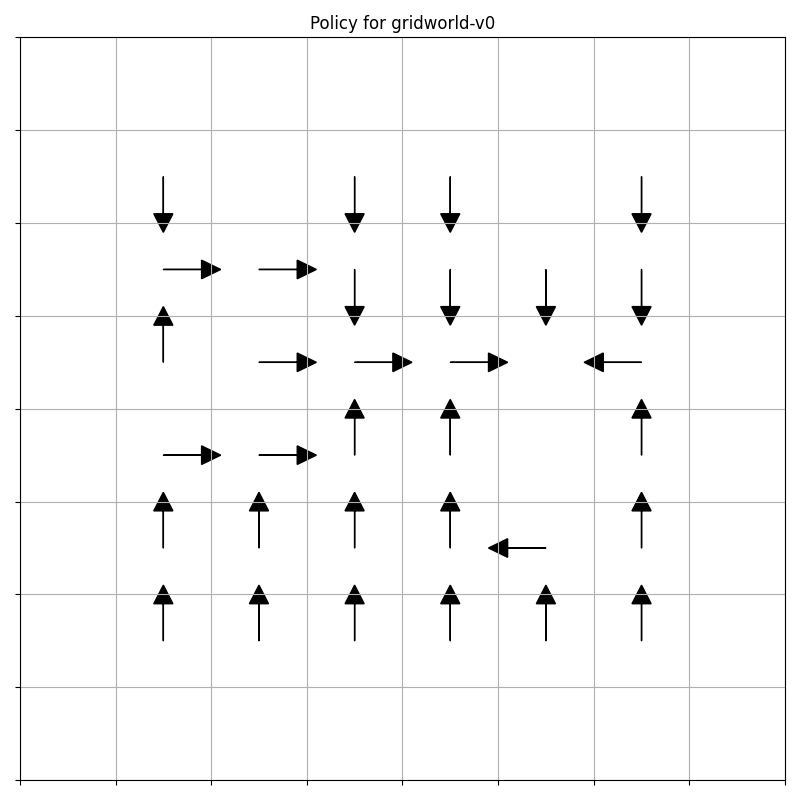
\includegraphics[scale=0.2]{hw4_rl/figures/gridworld-v0_deterministic_pi_gamma=0.99_policy}
\\
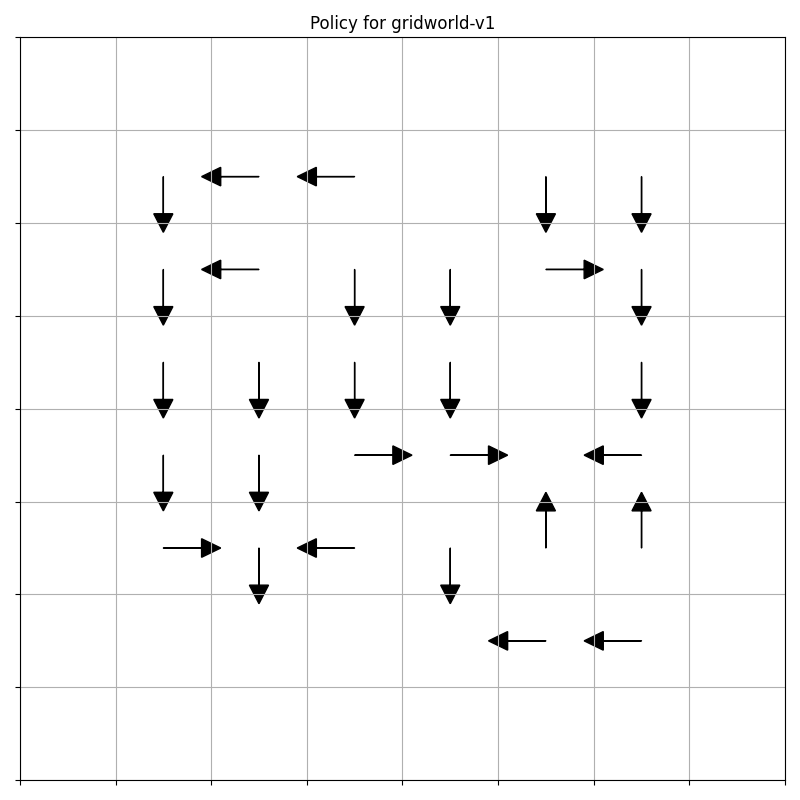
\includegraphics[scale=0.2]{hw4_rl/figures/gridworld-v1_deterministic_pi_gamma=0.5_policy} &
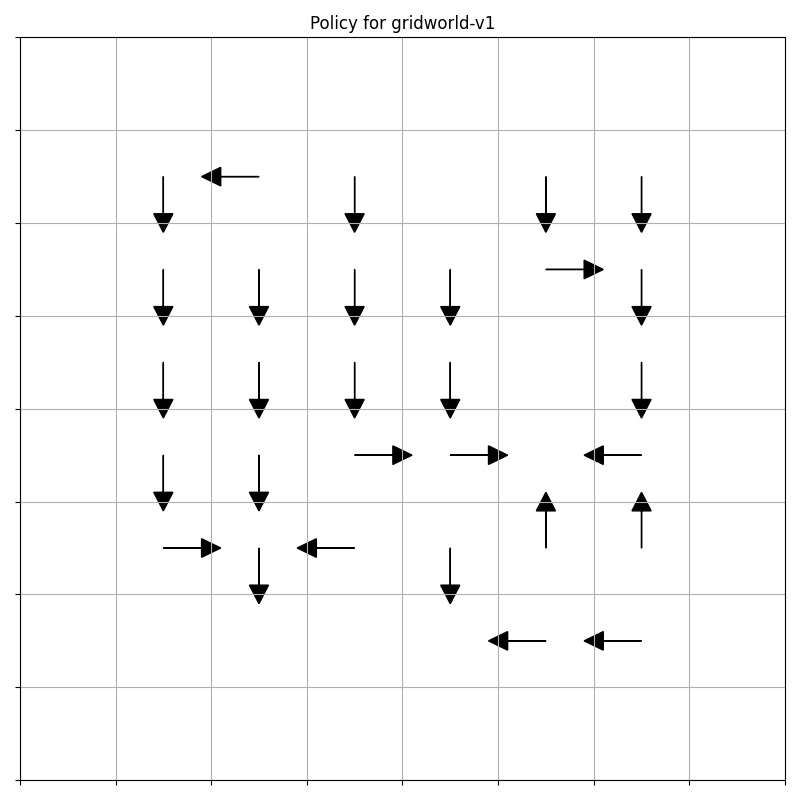
\includegraphics[scale=0.2]{hw4_rl/figures/gridworld-v1_deterministic_pi_gamma=0.75_policy} &
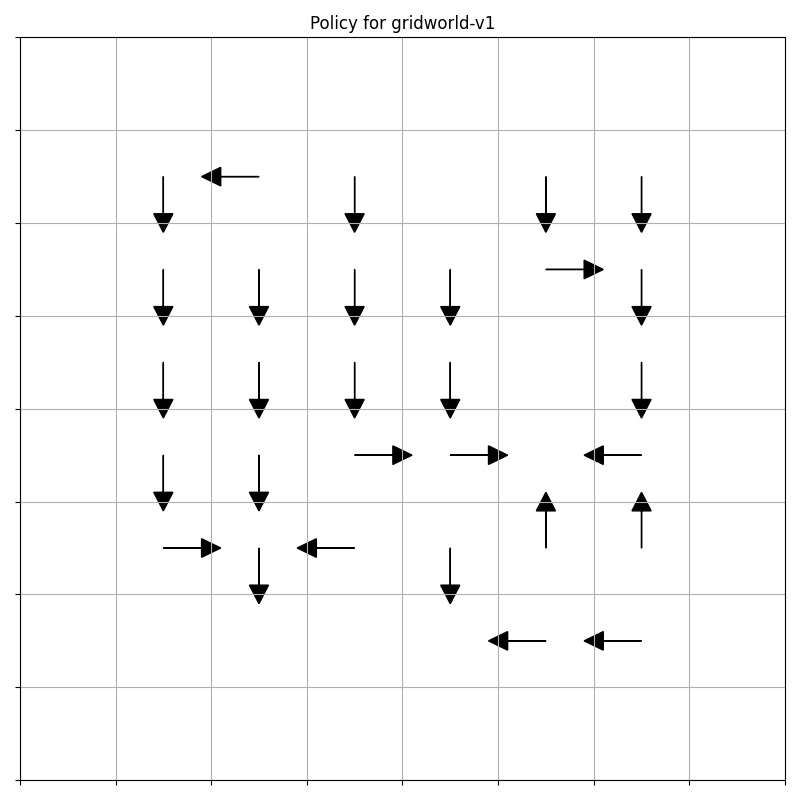
\includegraphics[scale=0.2]{hw4_rl/figures/gridworld-v1_deterministic_pi_gamma=0.9_policy} &
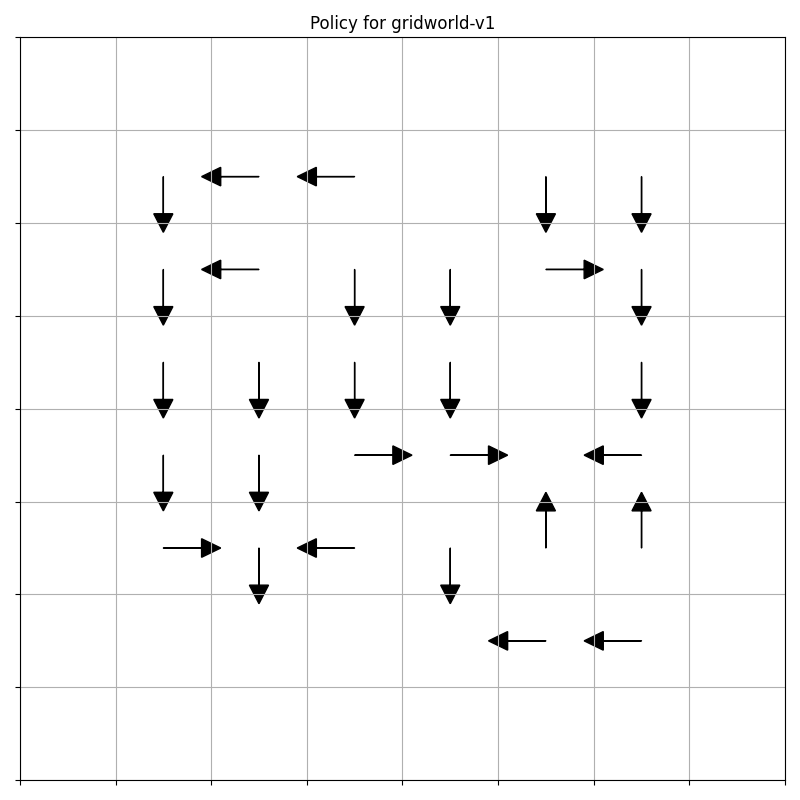
\includegraphics[scale=0.2]{hw4_rl/figures/gridworld-v1_deterministic_pi_gamma=0.99_policy}\\
$\gamma = 0.5$ & $\gamma = 0.75$ & $\gamma = 0.9$ & $\gamma = 0.99$
\end{tabular}
\caption{Policy for various values of $\gamma$}
\label{tab:policy_itteration_table}
\end{table}
As can be seen in the above table there is essentially no difference in policy regardless of the value for $\gamma$ used. This intuitively makes sense since there is no other lower reward state to be in. Thus even though there is no much look ahead the agent still moves to the square with the maximum reward as there is no other short sighted reward to be had. This would likely change however, if there was a lower reward state, such as adding a terminal state with +5 upon entry.\\
\newpage
This problem can also be solved exactly which will give the same results. As you can see below, the policy and value heat map is the same as the iterative method. See discussion below about the speed of this method vs the iterative methods. 
\begin{table}[H]
	\centering
	\begin{tabular}{cc}
		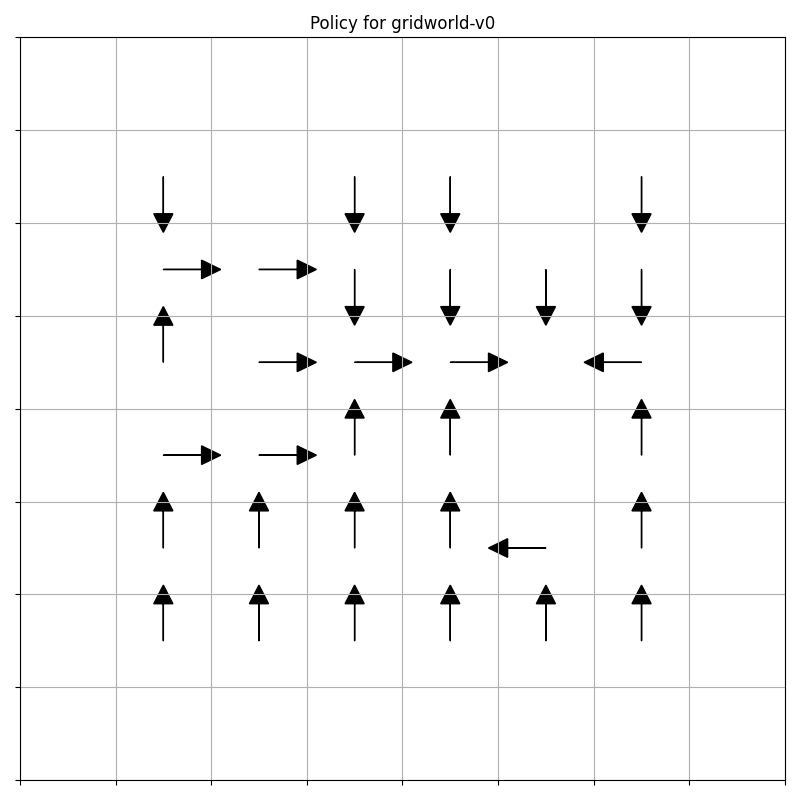
\includegraphics[scale=0.2]{hw4_rl/figures/gridworld-v0_deterministic_pi_gamma=0.99_policy} & 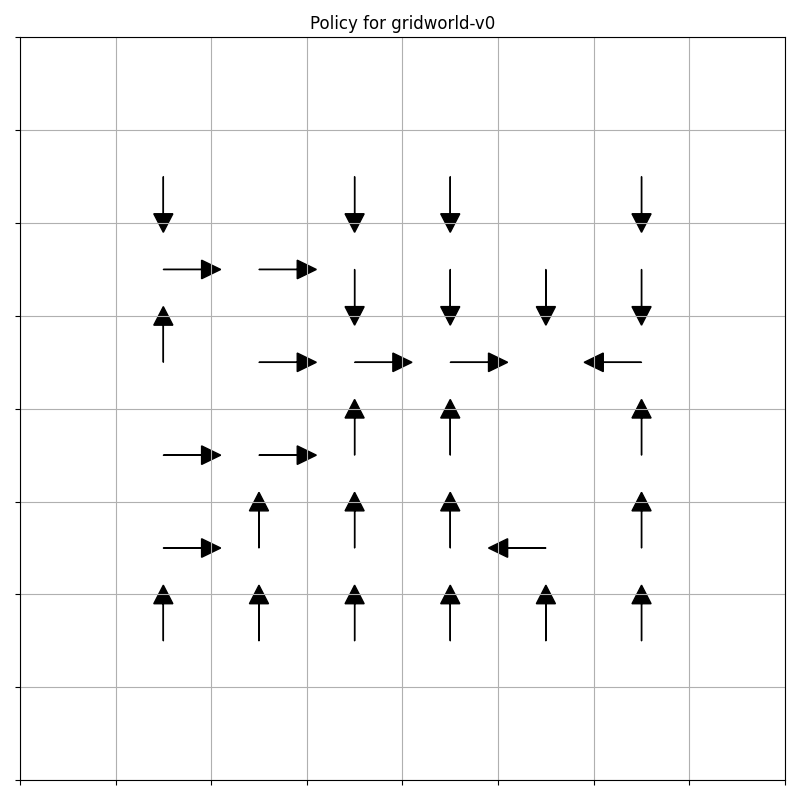
\includegraphics[scale=0.2]{hw4_rl/figures/gridworld-v0_exact_deterministic_pi_policy}\\
		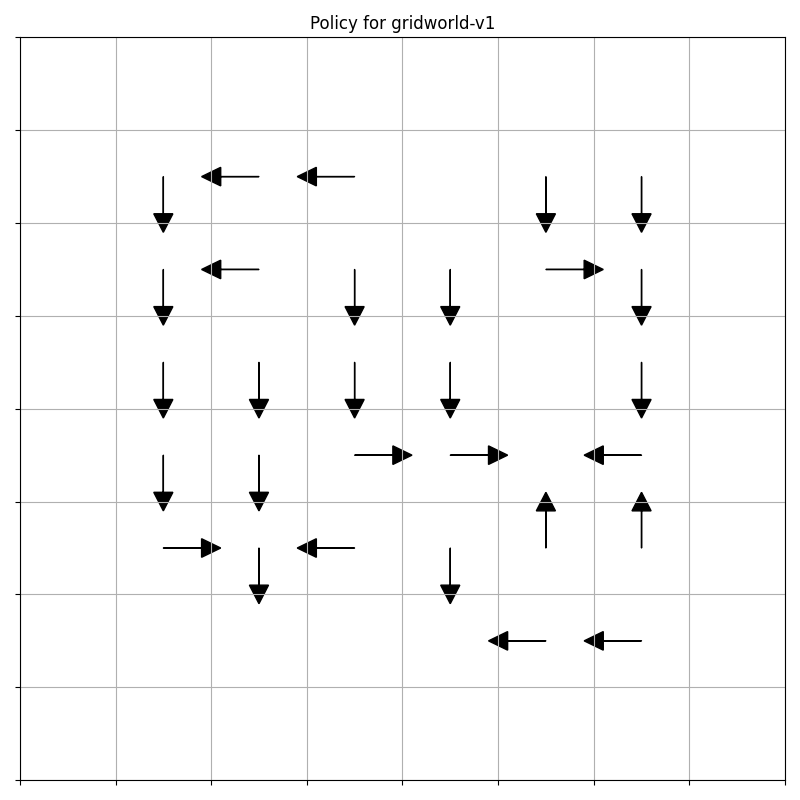
\includegraphics[scale=0.2]{hw4_rl/figures/gridworld-v1_deterministic_pi_gamma=0.99_policy} & 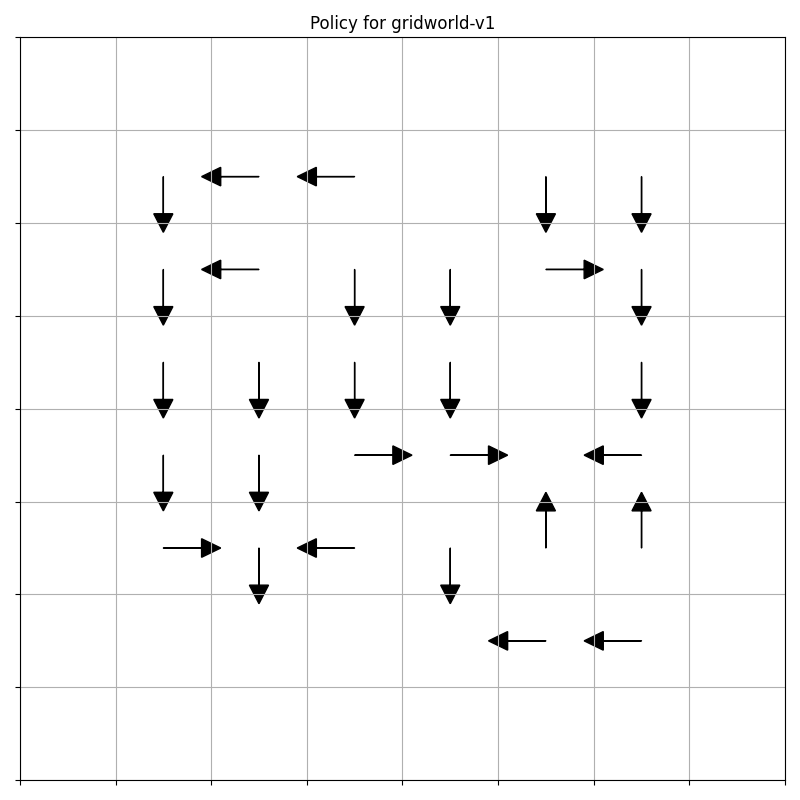
\includegraphics[scale=0.2]{hw4_rl/figures/gridworld-v1_exact_deterministic_pi_policy}\\
		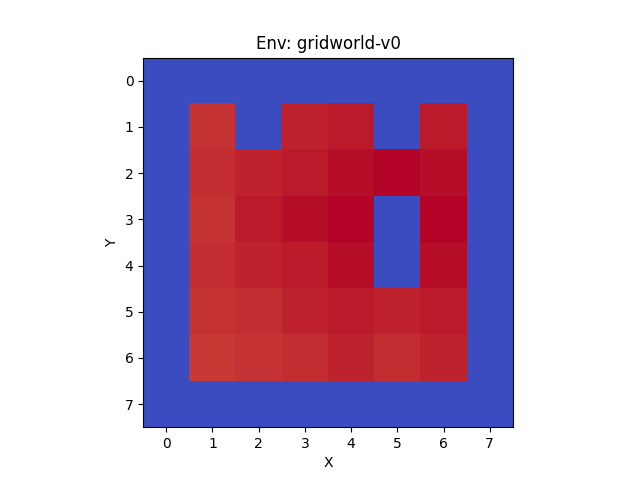
\includegraphics[scale=0.4]{hw4_rl/figures/gridworld-v0_deterministic_pi_gamma=0.99_value} & 
		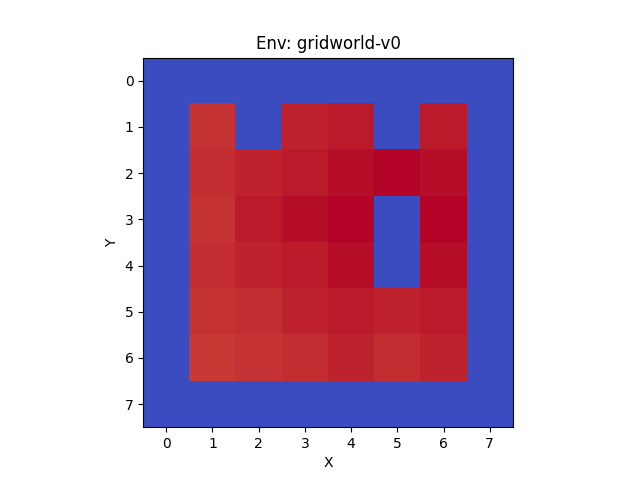
\includegraphics[scale=0.4]{hw4_rl/figures/gridworld-v0_exact_deterministic_pi_value}\\
		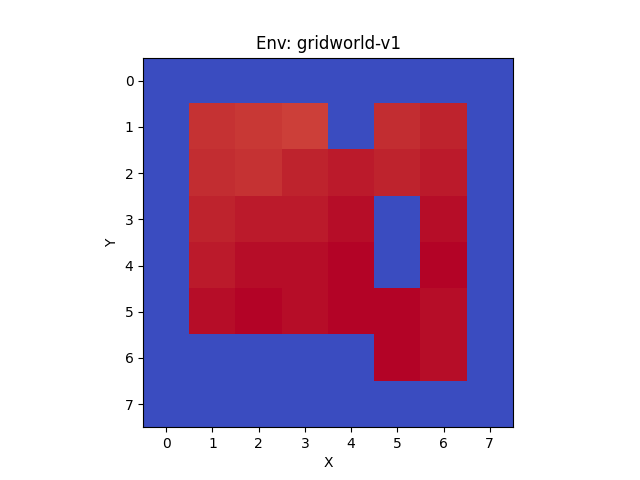
\includegraphics[scale=0.4]{hw4_rl/figures/gridworld-v1_deterministic_pi_gamma=0.99_value} &
		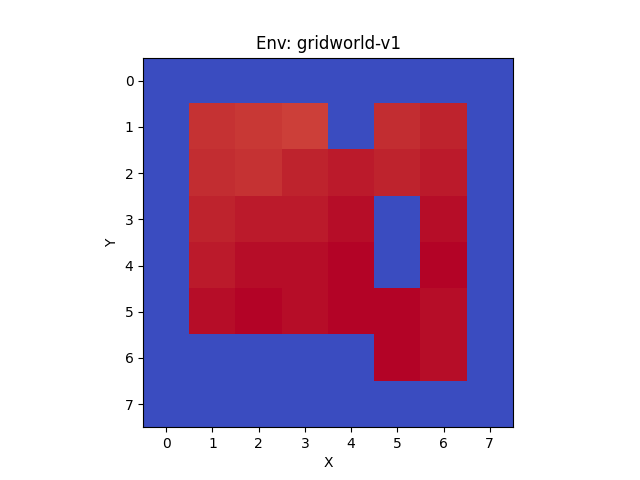
\includegraphics[scale=0.4]{hw4_rl/figures/gridworld-v1_exact_deterministic_pi_value}\\
		Iterative Policy Iteration & Exact Policy Solving
	\end{tabular}
	\caption{Difference between the value and heat map from solving exactly vs iteratively}
\end{table}
\newpage
\newcommand{\ViSTD}{0.0205}
\newcommand{\ViMean}{0.1760}
\newcommand{\PiSTD}{0.0108}
\newcommand{\PiMean}{0.1092}
\newcommand{\PiExactSTD}{0.0012}
\newcommand{\PiExactMean}{0.0061}

\section*{Value Iteration}
In the below table you can see the policy generated from policy iteration and value iteration, both have $\gamma=0.99$. 
\begin{table}[H]
	\centering
	\begin{tabular}{cc}
	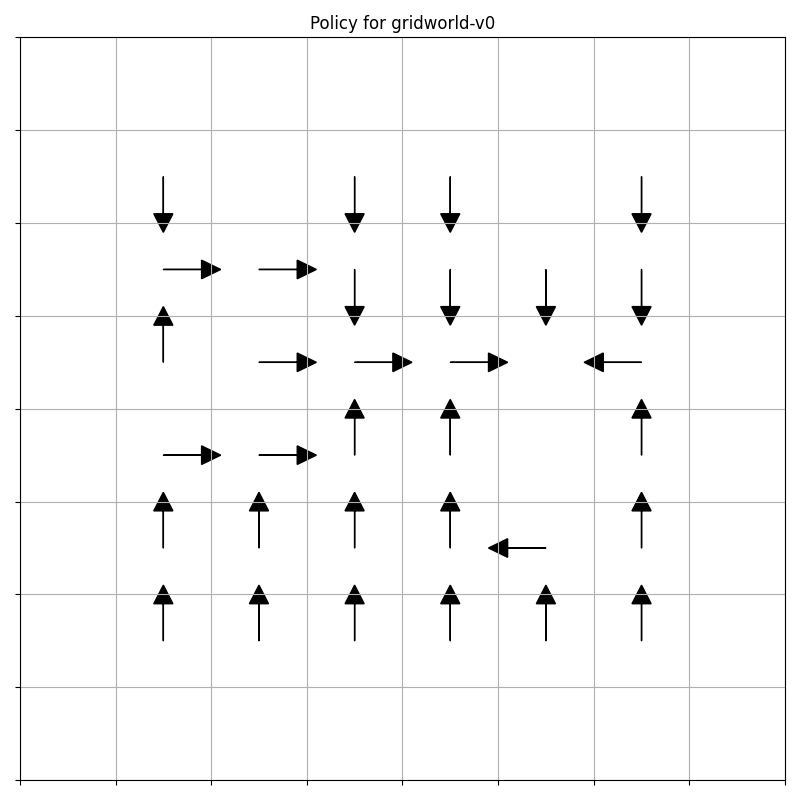
\includegraphics[scale=0.18]{hw4_rl/figures/gridworld-v0_deterministic_pi_gamma=0.99_policy} & 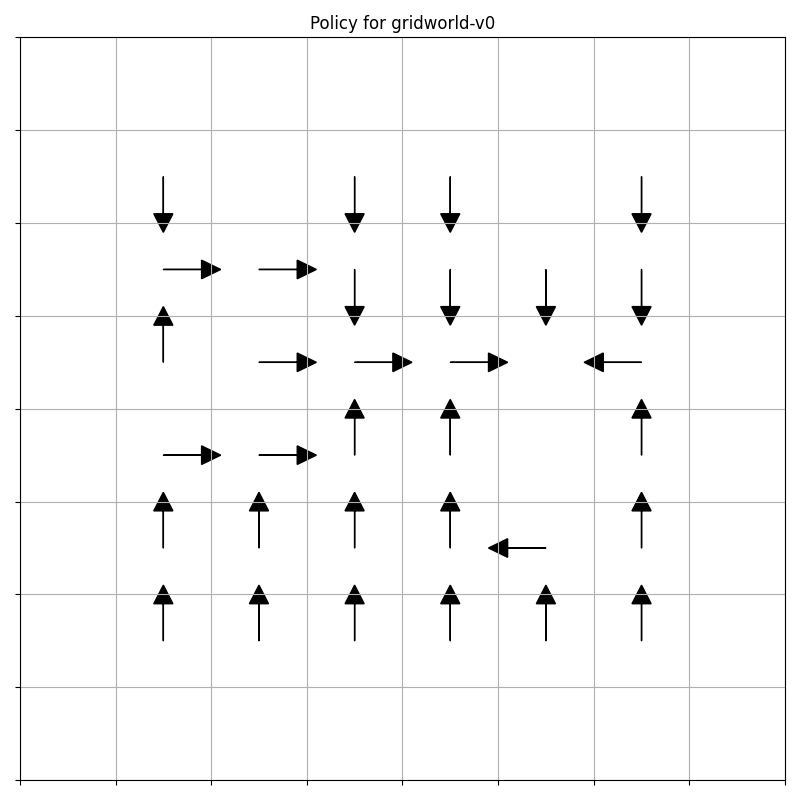
\includegraphics[scale=0.18]{hw4_rl/figures/gridworld-v0_deterministic_vi_policy}\\
	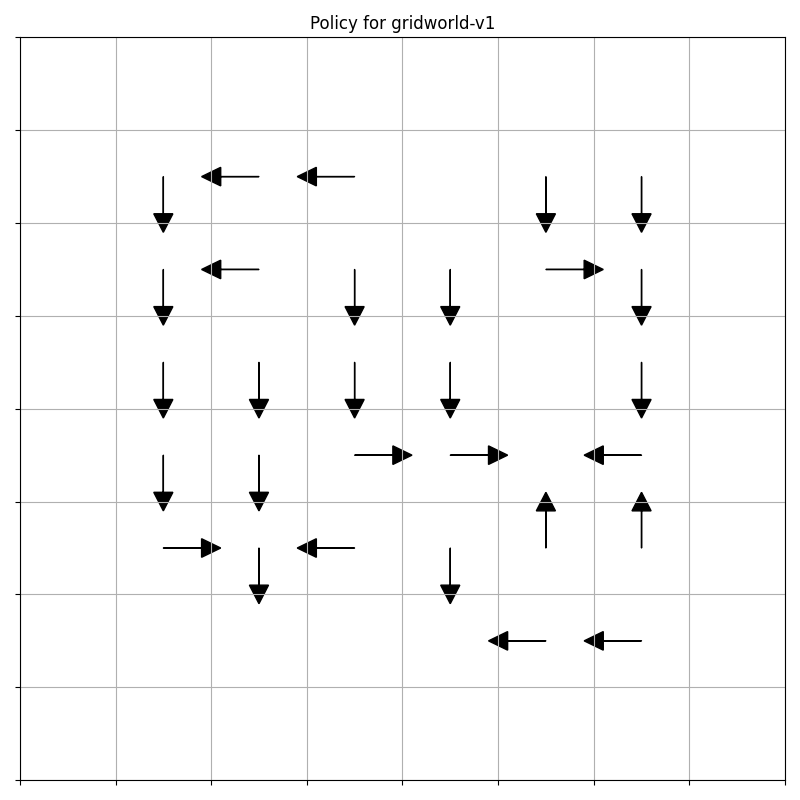
\includegraphics[scale=0.18]{hw4_rl/figures/gridworld-v1_deterministic_pi_gamma=0.99_policy} & 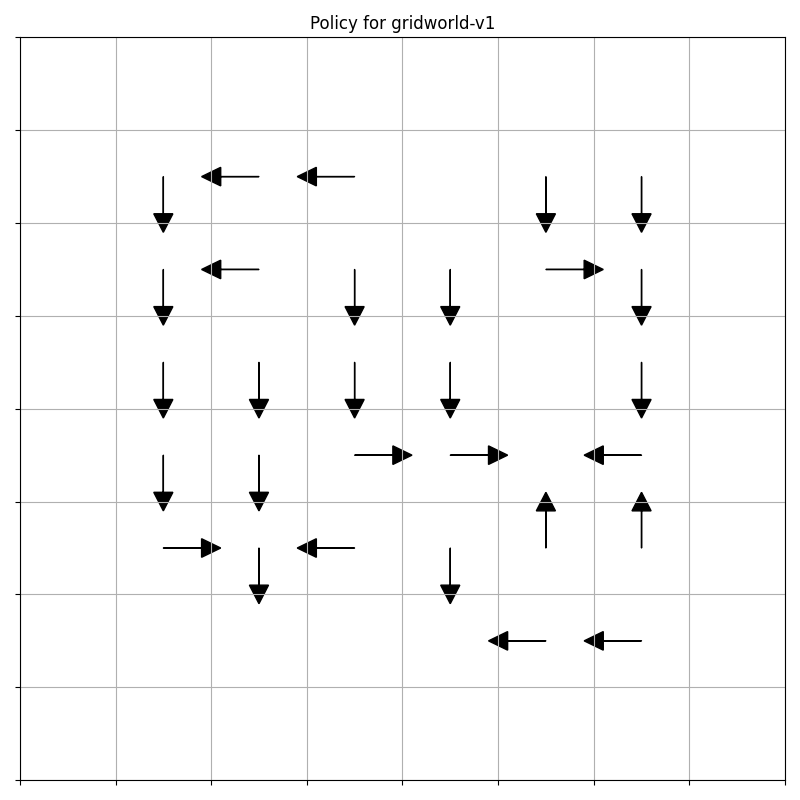
\includegraphics[scale=0.18]{hw4_rl/figures/gridworld-v1_deterministic_vi_policy}\\
	Policy Iteration & Value Iteration
	\end{tabular}
	\caption{Policy found via Policy Iteration vs Value Iteration}
	\label{tab:policy_vs_value_itteration_table}
\end{table}
As you can see in the above table both end up finding the same policy. This makes as policy and value iteration are just different ways of coming to same conclusion. 


Next looking at the computation time I ran each environment 100 times for policy and value iteration. Below is the plot with the mean times and standard deviation.
\begin{table}[H]
	\centering
	\begin{tabular}{ccc}
	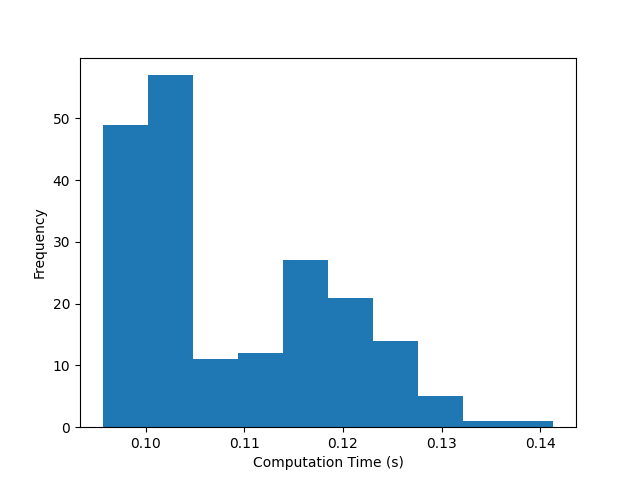
\includegraphics[scale=0.3]{hw4_rl/figures/pi_time_histogram}&
	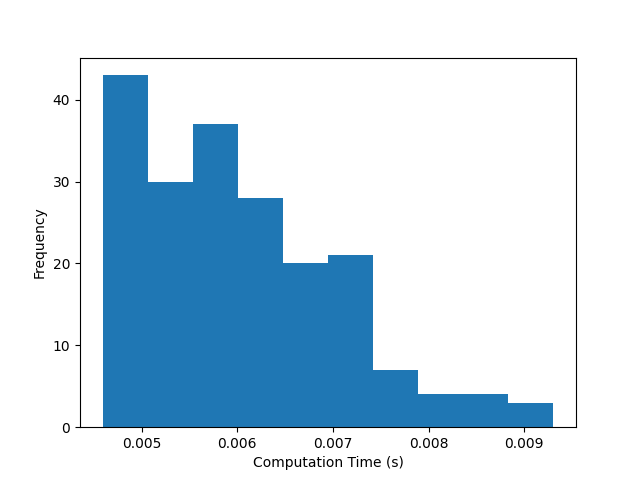
\includegraphics[scale=0.3]{hw4_rl/figures/exact_pi_time_histogram} & 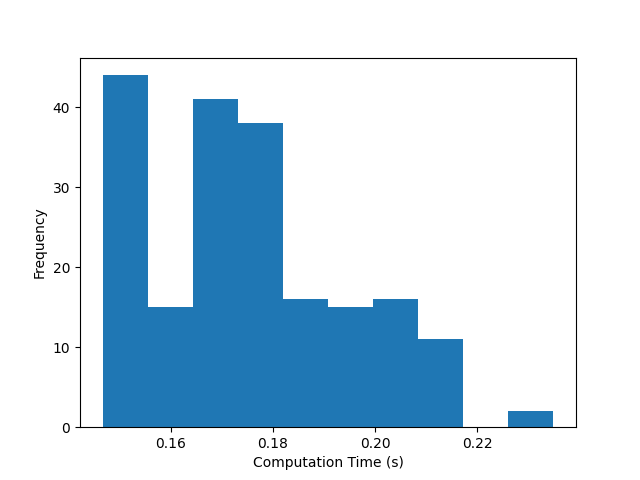
\includegraphics[scale=0.3]{hw4_rl/figures/vi_time_histogram} \\
	 Policy Iteration & Exact Policy  & Value Iteration\\
	 $\mu = \PiMean, \ \sigma=\PiSTD$ & $\mu = \PiExactMean, \ \sigma=\PiExactSTD$ & $\mu = \ViMean, \ \sigma=\ViSTD$
	\end{tabular}
	\caption{Time taken to compute policy for policy and value iteration}
\end{table}
As you can see by both the histogram and calculated statics both are pretty close with Policy iteration being slightly faster. This makes sense given that this is a pretty small MDP, which tends to lend policy iteration to have better performance. It is interesting to me how high the variance in time is though. Both polices were run back to back, on the same laptop, while it was plugged in so im not exactly sure why sometimes it takes longer that others to calculate the policy. \\

Now when looking at the exact solutions for policy this is significantly faster then either of the two iterative methods. This intuitively does make some sense since it only needs one step, and the algorithms for solving systems of linear equations are very robust and fast. However, overall this does not generalize to larger MDPs. If the environment was a lot bigger this would quickly become a much slower algorithm.
\newpage
\section*{Mountaineer}
\begin{table}[H]
	\centering
	\begin{tabular}{ccc}
		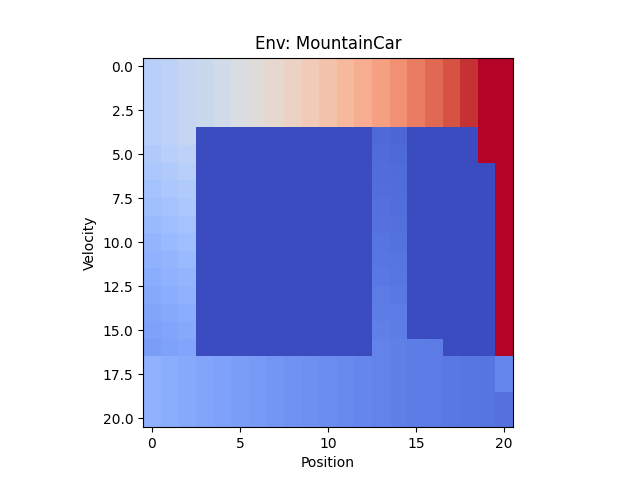
\includegraphics[scale=0.4]{hw4_rl/figures/mountaincar_deterministic_vi_value_21} & 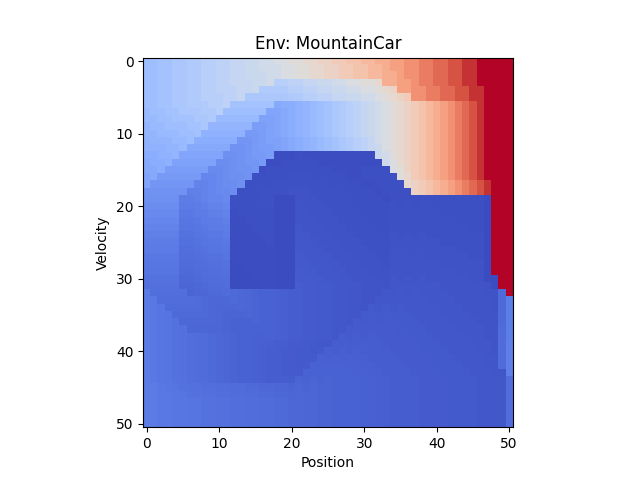
\includegraphics[scale=0.4]{hw4_rl/figures/mountaincar_deterministic_vi_value_51} & 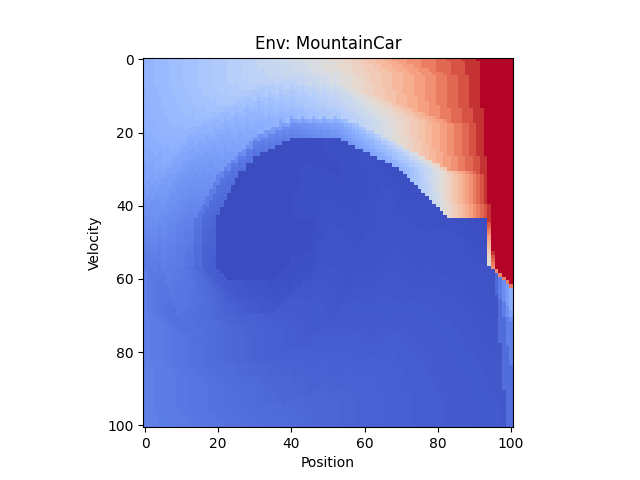
\includegraphics[scale=0.4]{hw4_rl/figures/mountaincar_deterministic_vi_value_101}\\
		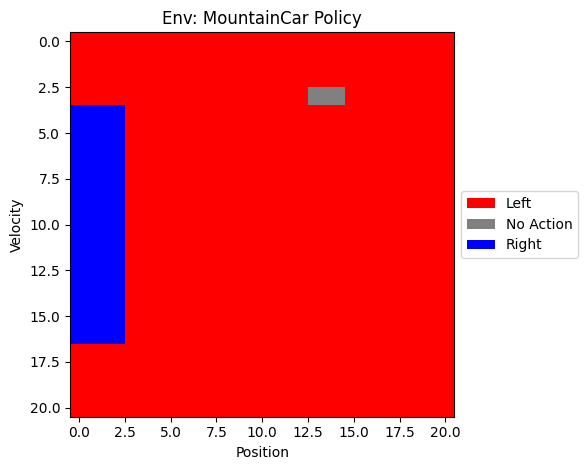
\includegraphics[scale=0.3]{hw4_rl/figures/mountaincar_deterministic_vi_policy_21} & 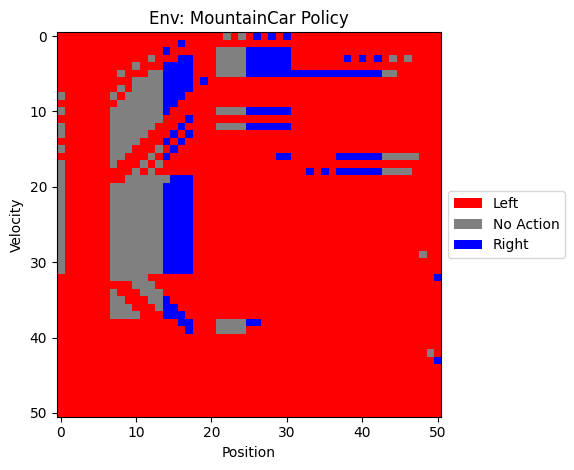
\includegraphics[scale=0.3]{hw4_rl/figures/mountaincar_deterministic_vi_policy_51} & 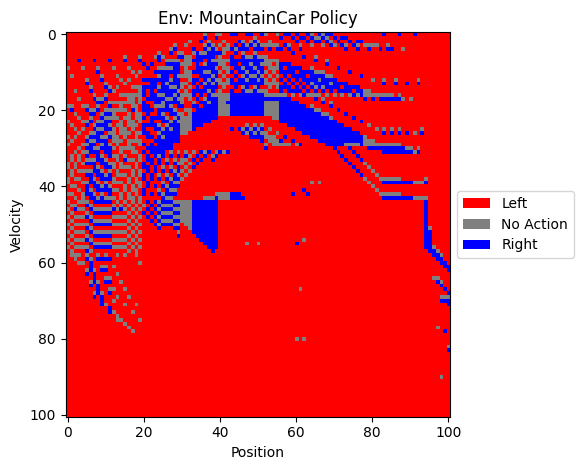
\includegraphics[scale=0.3]{hw4_rl/figures/mountaincar_deterministic_vi_policy_101}\\
		21 Bins & 51 Bins & 101 Bins
	\end{tabular}
\end{table}
\end{document}